\documentclass{article}
\usepackage{graphicx}
\usepackage{geometry}
\usepackage{hyperref}
\usepackage{mathtools}
\usepackage{float}
\graphicspath{{./}}
\geometry{a4paper, portrait, margin = 1in}
\title{1: Linear Regression Using Numpy}
\date{\today}
\author{Aniruddh K Budhgavi \\Enigma, IIIT-B}
\begin{document}
    \maketitle

    \section{Introduction}
        In machine learning, the two most common types of 
        problems we wish to solve are \textbf{regression} and 
        \textbf{classification}.
        \begin{itemize}
            \item \textbf{Regression:}
            \begin{itemize}
                \item Given some data points of the form $(x, y)$, where
                $x$ represents the input and $y$ is the output, (both are vectors),
                try to find a function $f(x)$ such that $f(x)$ is close to $y$ for all data points $(x, y)$.
                In simple terms, given data points $(x, y)$, try to find a plot that approximates 
                the relationship between $x$ and $y$ well.

                \item Example: Given the square footage of houses in a particular area 
                as well as the prices of the houses, try to find a function which can predict the 
                price of a particular house when the square footage is given.
            \end{itemize}
            \item \textbf{Classification:}
            \begin{itemize}
                \item Given some data points $x$, (vectors), where each $x$ belongs to a particular class,
                try to find a function which tells you which class a new point $x$ belongs to. In simple terms,
                given some data points which have been classified into groups, find a function which tells you which 
                class a given data point belongs to.

                \item Example: Given a bunch of photos, of which some are cat photos, try to find a 
                way of automatically classifying new photos as either cat photos or non-cat photos.
            \end{itemize}
        \end{itemize}

        A key point is that a regression or classification model should be able to predict the answer
        even for inputs \textbf{it has never seen before}. If this is still a little abstract,
        don't worry. The following exercise should make it quite clear.
    \newpage
    \section{Your First ML Model: Simple Linear Regression}
        \subsection{The code}
            \begin{itemize}
                \item You can find the implementation of this model at \href{https://github.com/aniruddhkb/enigmatutorials/blob/master/intro2ml/linearRegression.ipynb}{my github}.
                You will need Jupyter Notebooks as well as Numpy and Matplotlib to run this.
            \end{itemize}
        \subsection{Defining the problem}
            Let's say you have some data which looks like figure 1.
            \begin{figure}[h] \begin{center}
                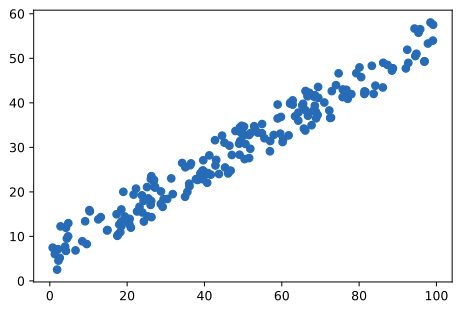
\includegraphics[width = 0.5\textwidth]{plot1.png}
                \caption{Our dataset. The inputs are on the x axis, and the corresponding outputs on the y axis.}
            \end{center} \end{figure}

            You wish to find the line which best fits this set of points.
            The model you can use to solve this problem is called a \textbf{linear regression model}.
            Specifically, this is a linear regression model where you have one input and one output
            for each data point -- the simplest case.
        \subsection{Some terminology}
            Throughout this series of articles, the following nomenclature will be consistently used.
            \begin{itemize}
                \item $m = $ The number of data points. Here, $m = 200$.
                \item $n_x = $ The number of inputs per point. Here, $n_x = 1$.
                \item $n_y = $ The number of outputs per point. Here, $n_y = 1$.
                \item $X = $ The matrix where each \emph{column} is one of $m$ data inputs.
                            Each column is $n_x$ long and there are $m$ such columns. Therefore,
                            this matrix is of dimension $(n_x, m)$.
                \item $Y = $ The matrix where each \emph{column} is one of $m$ data outputs.
                            Each column is $n_y$ long and there are $m$ such columns. Therefore,
                            this matrix is of dimension $(n_y, m)$.
            \end{itemize}
        \subsection{Starting off}
            \begin{enumerate}
                \item Every line in the 2-d plane is of the form
                \[
                    y = mx + c
                \]
                where $m$ and $c$ are parameters. This clashes with our existing nomenclature above.
                Therefore, throughout, we use
                \[
                    y = Wx + b  
                \]
                where $W$ is called the \emph{weight} and $b$ is called the \emph{bias}.

                \item Let us initialize $W$ and $b$ randomly. We know there exist $W_{optim}$ and $b_{optim}$
                such that the line $y = W_{optim}x + b_{optim}$ is a good fit for our data, but we do not know
                what their values are (yet).

                \item Now a question arises: How do we quantify how "good" the values we have chosen for $W$
                and $b$ are?
            \end{enumerate}
        \newpage
        \subsection{The cost function $J$}
            \begin{enumerate}
                \item Let us plot the data along with our line $y = Wx + b$. We get:
                \begin{figure}[h] \begin{center}
                    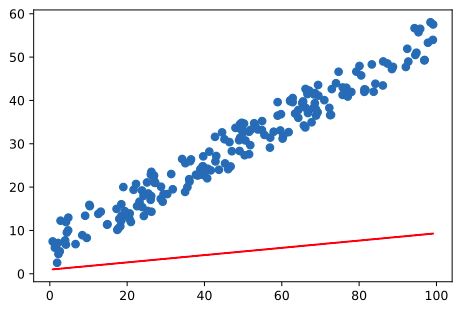
\includegraphics[width = 0.5\textwidth]{plot2.png}
                    \caption{Our data with our line}
                \end{center} \end{figure}
                \item Clearly, our line is a long way off from our data. But how do we quantify how "good" or "bad" the line is?
                \item Let's break this problem down even further. For a particular $x_i$ in our dataset, which has 
                a corresponding $y_i$, how do we know if our prediction $\hat{y}_i$ is close to $y_i$?
                \item A common way to quantify this is with the \textbf{square error}.
                \item Specifically, the loss for the i'th training example is:
                \[
                  L(\hat{y}_i, y_i) = \frac{1}{2}(\hat{y}_i - y_i)^2  
                \]
                where $\hat{y}_i$ is our \emph{prediction} for the i'th training example.
                \[
                  \hat{y}_i = Wx_i + b  
                \]
                What's nice about this is that if $\hat{y}_i$ and $y_i$ are far apart, then $L$ is very large,
                 and if $\hat{y}_i$ and $y_i$ are closer, then $L$ is very small.
                \item Now, the overall cost function $J$ for the whole dataset is 
                \[
                  J =  \frac{1}{m}\sum_{i = 1}^{m} L(\hat{y}_i, y_i) = \frac{1}{2m}\sum_{i = 1}^{m} (\hat{y}_i - y_i)^2  
                \]
                $J$ is the \textbf{mean square error} between $\hat{Y}$ and $Y$.
                \item Great! Now if we can just \emph{minimise} this cost function with respect to $W$ and $b$, our job is done.
            \end{enumerate}
        \subsection{Gradient descent}
            \begin{enumerate}
                \item How do we minimise a function with respect to an input variable? To examine this, let's
                have a look at a simpler function than $J$. Let's try to minimise 
                \[
                  y = \cos (x)  
                \]
                with respect to $x$.
                \item The way we learned to do this in twelfth standard is by taking the derivative, setting it equal 
                to zero, and solving. This is useful, but it is computationally expensive for higher dimensions.
                \item Let's plot the function.
                \begin{figure}[h] \begin{center}
                    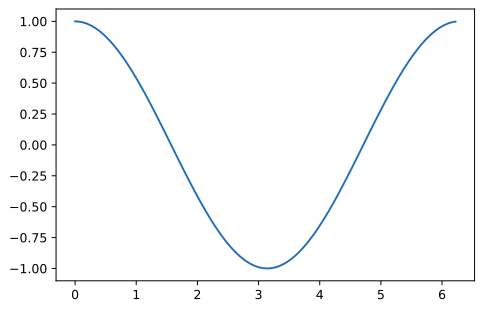
\includegraphics[width = 0.5\textwidth]{plot3.png}
                    \caption{The cosine function.}
                \end{center} \end{figure}
                \item Now, let's consider a particular point on this curve.
                \begin{figure}[H] \begin{center}
                    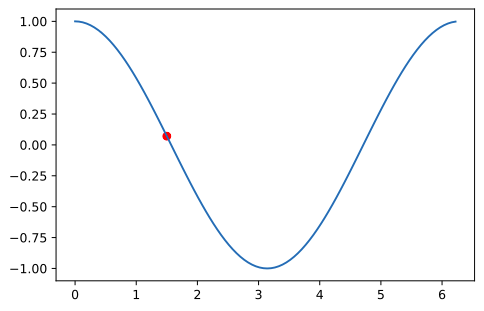
\includegraphics[width = 0.5\textwidth]{plot4.png}
                    \caption{The cosine function with a point.}
                \end{center} \end{figure}
                Observe that the slope of the function at this point is large and negative.
                \item Now, let's consider a different point on this curve.
                \begin{figure}[H] \begin{center}
                    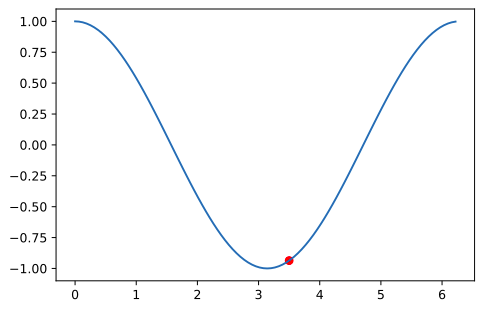
\includegraphics[width = 0.5\textwidth]{plot5.png}
                    \caption{The cosine function with a  different point.}
                \end{center} \end{figure}
                Observe that the slope of the function at this point is small and positive.
                \item If we are at a point to the right of the minimum, the slope is positive.
                If we are at a point to the left of the minimum, the slope is negative.
                For points close to the local minimum, the slope is small.
                For points farther from the local minimum, the slope is large (in general).
                \item In other words, if we move in the direction of the \textbf{negative of the 
                slope} at a point, we will move towards the local minimum.
                \item Starting from an arbitrary $x$, we will move closer to the local minimum by doing:
                \[
                    x \coloneqq x - \alpha\frac {d \cos x}{dx} 
                \]
                where $\alpha$, the \textbf{learning rate}, is a small positive float, like $0.1$ or $0.01$. By running the above assignment
                many times, $x$ will gradually converge to the point of local minimum.

                \item This is called \textbf{gradient descent}. Applying gradient descent to $J$ with respect to $W$ and $b$,
                we get
                \[
                    W \coloneqq W - \alpha \frac {\partial J}{\partial W}
                    \\
                    b \coloneqq b - \alpha \frac {\partial J}{\partial b}  
                \]
                The partial derivatives are to emphasise that the derivatives are taken keeping the other terms constant.
                When taking the derivative wrt $W$, we assume that $b$ is constant, and when taking the derivative wrt $b$, we assume that $W$ is constant.
                \item Applying gradient descent, say, 1000 or 10,000 times, we would get optimal values of $W$ and $b$.
                \item Now to calculate the derivatives:
                \[
                    J = \frac {1}{2m} \sum _{i = 1}^{m} (Wx_i + b - y_i)^2 \\
                    \frac {\partial J}{\partial W} = \frac {1} {m} \sum _{i = 1}^{m} x_i(Wx_i + b - y_i) \\
                    \frac {\partial J}{\partial b} = \frac {1} {m} \sum _{i = 1}^{m} (Wx_i + b - y_i)  
                \]
                Plug these back into the gradient descent rule above, run it , say, a few thousand times or so, and have a look at the results.
            \end{enumerate}
        \subsection{Results}
            \begin{enumerate}
                \item Let's now see the graph for $ y = Wx + b$ superimposed on our data.
                \begin{figure}[h] \begin{center}
                    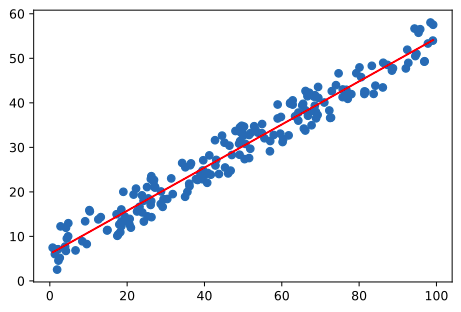
\includegraphics[width = 0.5\textwidth]{plot9.png}
                    \caption{The results. We used $\alpha = 0.005$ and 100,000 iterations.}
                \end{center} \end{figure}
                Looks pretty good, right?
                \item Another common practice is to plot the cost function $J$ as a function of the number of iterations.
                \begin{figure}[H] \begin{center}
                    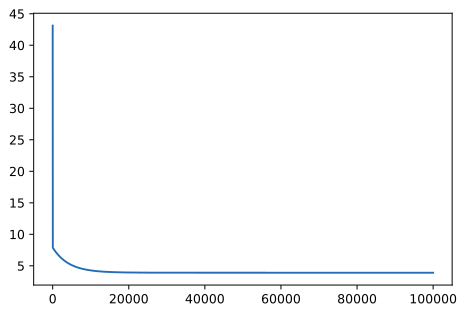
\includegraphics[width = 0.5\textwidth]{plot10.png}
                    \caption{The cost function over iterations.}
                \end{center} \end{figure}
                \item \emph{Sometimes}, gradient descent won't work as you expect it to. The cost function blows up exponentially. Assuming your equations are correct,
                the reason for this is that your learning rate $\alpha$ 
                is too large. If your learning rate is too large, you will "overshoot" the minimum and gradient descent will fail to converge.
                Reduce $\alpha$ by an order of magnitude or two and try again. Of course, with a smaller alpha, the number of iterations needed will be large.
            \end{enumerate}
        \subsection{Additional practice}
            \begin{enumerate}
                \item You can find two datasets \href{https://github.com/aniruddhkb/enigmatutorials/tree/master/intro2ml/linearRegression}{here}.
                \item The files are .csv -- you'll have to figure out how to import them as Numpy arrays and use them.
            \end{enumerate}
        \subsection{Looking ahead}
            \begin{enumerate}
                \item In general, $x_i$ need not be a scalar -- it can be a vector too. The same applies to $y_i$ as well.
                \item The only difference is that $W$ and $b$ are not scalars. $W$ is a matrix and $b$ is a vector. You should be able to
                find the dimensions of $W$ and $b$ based on the information provided at the very beginning about the dimensions of $x_i$ and $y_i$.
                \item Congratulations! You have just built your first ever machine learning model! Linear regression, while simple in theory, is actually a 
                very powerful tool and is often sufficient for many applications.
                \item Next time, we will learn about \textbf{logistic regression}.
            \end{enumerate}
            
            
\end{document}}